% Este archivo es parte de la memoria del proyecto fin de carrera
% de Aarón Bueno Villares. Protegida bajo la licencia GFDL.
%
% Para más información, la licencia completa viene incluida en el
% fichero fdl-1.3.tex

% Copyright (C) 2010 Aarón Bueno Villares

\chapter{Desarrollo del sistema}
\label{chap:desarrollo}

El primer paso mas importante antes de comenzar a crear verdaderamente
\gomf, es planificar su desarrollo, indentificando sus partes, y,
sobre todo, forjar definitivamente qué vamos a entender por \gomf, es
decir, qué hará exáctamente y cómo, y de cara al usuario, \gomf.

La búsqueda de la respuesta a esta pregunta ha sido el mas fiel
acompañante del proceso de desarrollo, pues no terminó de contestarse
hasta su finalización, pues como ya advierte la ingeniería del software, esta
tarea no es nada sencilla. Y además, cuando a uno se le ofrece la
oportunidad de \emph{hacer lo que  quiera}, solo un conformista se
declarará impasible ante esta situación. Es una vía abierta para
desplegar sus artes y de demostrar a los demás, como excusa para
demostrarse a sí mismo, sus propias capacidades. En este punto, las
ideas flotan, emergen y nadan en un mar caótico de realizaciones
personales a las que difícilmente se les puede poner orden.

El proceso de diseño y la implementación consecuente se fue realizando
a medida que se aclaraba la respuesta a la primera pregunta. Por
tanto, podemos decir que nuestro proyecto se ha realizado bajo una
modelo de desarrollo iterativo incremental, donde, por lo general, a
cada nueva iteración se definían (o redefinían) los siguientes
aspectos a desarrollar, junto a la experiencia ganada en los ciclos
anteriores. También el propio reglamento fue adaptándose a las
dificultades encontradas en el diseño y la implementación. La
descripción en esta memoria del proceso de desarrollo reflejará esta
historia.

La orientación a objetos ha sido el enfoque elegido para realizar el
desarrollo de nuestro juego.

\newpage
% Este archivo es parte de la memoria del proyecto fin de carrera
% de Aarón Bueno Villares. Protegida bajo la licencia GFDL.
%
% Para más información, la licencia completa viene incluida en el
% fichero fdl-1.3.tex

% Copyright (C) 2010 Aarón Bueno Villares

\section{Calendario}
\label{sec:calendario}

Aquí se describirá mas concisamente el contenido de cada una de estas
iteraciones de desarrollo.

Hay que advertir que durante todo el tiempo que ha
durado la confección de este proyecto no me he dedicado únicamente al
mismo. Mientras, continuaba las asignaturas que me quedaban de la
titulación técnica y luego comencé a cursar asignaturas del segundo
ciclo. Así que, en muchas ocasiones durante la realización del
proyecto me he visto obligado a pausar el desarrollo del mismo para
dedicarme enteramente a las asignaturas, lo que explica en parte su
larga duración.

En la figura \ref{fig:gantt} se muestra el diagrama de Gantt
correspondiente al calendario de nuestro proyecto.

\subsection{Definición inicial}
Cuando decidí realizar este proyecto, solo tenía una idea vaga de qué
iba a desarrollar. Tenía un propósito y un objetivo, como ya se
advirtió en el capítulo \ref{chap:introduccion}, pero no
sabía de que forma concreta esas ideas tomarían definitivamente
su forma. El primer ciclo de desarrollo corresponde a este periodo de
reflexión inicial, que fecundó en un reglamento que serviría como
punto de partida para el desarrollo consecuente.

En esta iteración se definió la categoría del juego, tras conocer e
investigar los taxones en los que se clasifican los videojuegos, se
conoció algo de la historia del paradigma de juegos de mesa que estaba
implementando para obtener inspiración de diversos reglamentos de
diversos juegos históricos de táctica militar (aunque mi mayor fuente
de inspiración siempre ha sido el reglamento de \emph{WF} por
ser el reglamento que mejor conozco), y se exploró mas concisamente
acerca de si efectivamente mi juego sería el único videojuego de esta
corte, explorando muchas páginas webs dedicadas a la recopilación de
información sobre videojuegos tanto clásicos como modernos. Así que
podemos decir que este primer ciclo también contiene una etapa de
documentación.

También se estuvo decidiendo que \emph{paradigma} de interfaz
usaríamos, si el videojuego sería 3D, isométrico o un juego 2D
plano. Al final me decanté por la última opción, pues no tenía las
artes suficientes para crear los modelos gráficos que necesitaría para
las dos primeras opciones.

Por último, junto a los demás aspectos, se configuró un reglamento
inicial de \gom.

\subsection{Arquitectura general del sistema}
Esta iteración contituye el primer ciclo de diseño, que a su vez es el mas
importante, pues se estableció la arquitectura general del sistema
(véase \ref{sec:diseno}), es decir, como organizaríamos las clases
principales y de mas alto nivel de abstracción que conformarían la
resolución del problema de implementar ese primer reglamento.

\subsection{Fase de movimiento}
La primera fase que se diseñó y luego implementó fue la fase de
movimiento. En su intento de implementación, se rediseñó el reglamento
en gran medida, pues llegé a comprender la gran complejidad que
contenía la versión inicial. Este ciclo contituye casi el 80\% del
desarrollo del sistema, sobre todo por las dificultades en establecer
los cálculos correctos del \emph{gestor de escenarios} (véase
\ref{sec:diseno}), que contenía mucha matemática y geometría.

\subsection{Gestor de interfaz}
Conjuntamente al ciclo anterior, se fue implementando la interfaz
necesaria para poder visualizar las implementaciones del gestor de
movimiento. Esta primera versión del gestor de interfaz fue la que
configuró el aspecto gráfico de las batallas.

\subsection{Fase de combate}
Una vez implementada la fase de movimiento, se podía comenzar a
desarrollar la fase de combate, pues sin la primera, no se podía
desarrollar la segunda (para combatir, hace falta realizar
cargas, cosa que se hace en la fase de movimiento). Nuevamente, el
reglamento sufrió modificaciones en torno a los aspectos involucrados
en esta fase.

\subsection{Mejora de la interfaz}
En esta iteración o ciclo, el gestor de interfaz tomaría su forma
final. Ya no sería un simple \emph{visualizador de batallas}. Ahora
sería una interfaz de menús donde el usuario podía realizar varias
cosas, no solo jugar batallas.

Por ello, se añadió una herramienta para poder configurar ejércitos
desde el propio programa, que luego se podrían elegir desde el mismo
software para comenzar la partida. La creación de esta herramienta
propició una nueva linea de desarrollo que tiene autonomía por sí
misma.

También se dedicó un episodio importante a mejorar
la interfaz gráfica, añadiendo multitud de cambios, a ajustar las
fuentes, las imágenes, los ejércitos y los sonidos, y a realizar
modificaciones en la interfaz para adaptar los nuevos cambios e ideas.

\subsection{Fase de disparos y magia}
En esta iteración, se añadió al juego la fase de disparo, y también se
implementó la magia. La inclusión en el juego de los disparos y la
magia fue bastante sencilla, quizás gracias al buen diseño realizado en las
iteraciones anteriores.

\subsection{Memoria del proyecto}
Una vez terminado de programar el juego, se hizo la memoria del
proyecto. En realidad, esta memoria ya había ido realizándose
paulatinamente junto a las iteraciones anteriores, pero tras finalizar el
juego fue cuando me dediqué enteramente a su confección.

\begin{figure}[h]
  \centering
  \includegraphics[scale=.5]{./imagenes/Gantt.png}
  \caption{Diagrama de Gantt del calendario del proyecto}
  \label{fig:gantt}
\end{figure}

\cleardoublepage

% Este archivo es parte de la memoria del proyecto fin de carrera
% de Aarón Bueno Villares. Protegida bajo la licencia GFDL.
%
% Para más información, la licencia completa viene incluida en el
% fichero fdl-1.3.tex

% Copyright (C) 2010 Aarón Bueno Villares

\section{Especificación de requisitos del sistema}
\label{sec:ers}

\subsection{Introducción}

Esta sección es una \emph{Especificación de Requisitos Software} (ERS) para el videojuego 2D de táctica militar basado en turnos, basado en reglamento y de corte medieval-fantástico \gomf. Esta especificación ha sido elaborada bajo el marco diseñado por el estándar \emph{IEEE Recommended Practice for Software Requirements Specification ANSI/IEEE 830 1998}.

\subsubsection{Propósito}
\label{sec:proposito}
El propósito de esta especificación es fundamentar las bases funcionales de \gomf. Está orientado tanto a los usuarios del sistema como a futuros desarrolladores. Esta especificación está sujeta a revisiones durante el ciclo de vida del producto, según las nuevas exigencias por parte de los usuarios finales, según posibles futuras inconsistencias o carencias, así como por los posibles caprichos de adición de funcionalidades por parte de el/los desarrollador/es.

\subsubsection{Alcance}
\label{sec:proposito}

\paragraph{\gomf}
\gom es un videojuego libre 2D de táctica militar por turnos y de corte fantástico-medieval (free fantasy turn-based tactics 2D-videowargame), de licencia GPL, y basado en reglamento (especificación estricta de todas las acciones posibles).

Está inspirado fuertemente en \textit{Warhammer Fantasy Battles} -de una alta vitalidad en el mercado-, un juego del mismo género, pero de mesa y con miniaturas, propiedad de la empresa inglesa Games Workshop.

\paragraph{Objetivos}
Este proyecto abarca la misión principal de desarrollar una alternativa digital, libre y gratuita, y si es posible, mejorada, del paradigma de juego cuyo máximo representante es \textit{Warhammer Fantasy Battles}.

No tiene como objetivo ser un juego de amplia difusión, ni con pretensiones de seducir a cualquier usuario potencial. Sus pretensiones van mas bien encaminadas a satisfacer las necesidades de jugadores que ya conocen dicho paradigma o para entusiastas de la táctica en general. Lo mas probable es que, para un jugador medio, el juego le parezca de lo mas artificial.

\paragraph{\emph{¿Qué hace y qué no hace el producto?}}
Esta pregunta se responde de la siguiente manera:
\begin{enumerate}
\item \gom no es un juego de estrategia, es un juego táctico.

La diferencia entre la táctica y la estrategia es difusa. La estrategia hace referencia a un propósito general, y la táctica al método para un fin específico. Estrategia es organizar una campaña militar en el lejano oriente. Táctica es un conjunto de movimientos específicos para ganar una batalla concreta, en la vida de dicha campaña. \gom se adentra en la segunda categoría.
 
\item \gom no es un juego de rol.

En los juegos de rol, el juego se organiza entorno a un personaje o conjunto reducido de personajes, que tienen una personalidad, un propósito y unas características. Mediante un conjunto de atributos, se modela toda la cosmovisión del/los personaje/s.

En \gomf, cada partida es independiente, y, aunque los distintos efectivos de cada unidad tengan atributos específicos que la modelan, la experiencia y posibles mejoras del usuario no tendrán efecto ninguno en el juego. \gom no distinguirá si un usuario es novato o un experto comandante, y la ejecución de una partida no tendrá efectos en la ejecución de partidas futuras, ni dependerá del éxito en partidas anteriores.

\item \gom no es un juego de tablero.

Un juego de tablero está basado en fichas que se desplazan sobre una
superficie organizada en casillas. \gomf, sin embargo, está mas bien un juego basado en elementos (unidades y efectivos) que pueden posicionarse en cualquier lugar de la ``mesa de juego''. Esto significa que los movimientos son completamente libres, y no están restringidos a movimientos en cantidades discretas, ni a posicionamiento en casillas.

\textit{Fantasy Wars} es el juego mas similar que he podido encontrar a \gom, pero está basado en un tablero tipo colmena (casillas hexagonales), y el jugador de ese modo ve limitada sus posibilidades de movimiento.

\end{enumerate}

\subsubsection{Visión general}
Esta ERS está organizada en tres subsecciones, a saber:
\begin{itemize}
\item  \textit{Introducción}: Es la subsección que en este momento
  estás leyendo. Explica qué es el producto y las directrices generales del documento.
\item \textit{Requisitos generales}: Se da una visión global del
  contexto funcional del producto: hardware y software implicado, así
  como la funcionalidad de mas alto nivel.
\item \textit{Requisitos específicos}. Se muestran, en concreto, cada una de las funcionalidades implicadas en el sistema.  
\end{itemize}

\subsection{Requisitos generales}
\subsubsection{Perspectiva del producto}
\begin{itemize}
\item \gom no pertenece a ningún producto mayor ni es parte de ningún otro software.
\end{itemize}

\subsubsection{Funciones del juego}
\begin{itemize}
\item La función principal del juego es permitir el enfrentamiento entre dos ejércitos, cada uno comandado por un usuario humano, según el reglamento de \gomf.
\item El usuario podrá crear su propio ejército.
\end{itemize}

\subsubsection{Características de los usuarios}
\begin{itemize}
\item Los usuarios que comanden cada ejército en una batalla deberán estar presentes en la misma máquina en la que se ejecute el juego.

\item Una vez los usuarios conozcan superficialmente el reglamento (las reglas mas generales), no tendrán problemas en habituarse velozmente y de forma intuitiva al uso del juego.
\end{itemize}

\subsubsection{Restricciones}
\begin{itemize}
\item El software tendrá una licencia libre, y en concreto, correrá bajo los derechos recogidos por la licencia GPL (GNU Public License).
\item Toda biblioteca usada para la implementación de este proyecto deberá ser multiplataforma.
\end{itemize}

\subsubsection{Suposiciones y dependencias}
Se asume que todos los requisitos descritos en esta especificación son consistentes e inmutables para la versión actual del producto. Todo posible cambio o modificación futura generará indefectiblemente una nueva versión del producto. La versión del producto actual es la 1, y será, asimismo, la versión de esta especificación así como la versión del documento de diseño generado a partir de esta especificación.

Si se propone una ampliación de los requisitos del sistema, sin modificar los existentes, se generará indefectiblemente una nueva subversión del producto. La subversión actual es la 1.0, y será, asimismo, la subversión de esta especificación así como la subversión del documento de diseño generado a partir de esta especificación.

\subsection{Requisitos específicos}

\subsubsection{Requisitos de interfaz externa}

\requisito{requisitos/interfazusuario}
\requisito{requisitos/interfazhardware}
\requisito{requisitos/velocidadreaccion}
\requisito{requisitos/resolucionpantalla}
\requisito{requisitos/sonido}

\subsubsection{Requisitos funcionales}

\requisito{requisitos/comenzarbatalla}
\requisito{requisitos/crearejercito}
\requisito{requisitos/editarejercito}
\requisito{requisitos/salir}
\requisito{requisitos/modificarejercito}
\requisito{requisitos/elegirraza}
\requisito{requisitos/informaciontarea}
\requisito{requisitos/ejecutartarea}

\subsubsection{Requisitos de rendimiento}

\requisito{requisitos/tiempo}
\requisito{requisitos/memoria}

\subsubsection{Restricciones de diseño}

\requisito{requisitos/enfoqueOO}
\requisito{requisitos/estandardiseno}

\subsubsection{Atributos del sistema software}

\requisito{requisitos/completitud}
\requisito{requisitos/documentacion}
\requisito{requisitos/escalabilidad}
\requisito{requisitos/portabilidad}
\requisito{requisitos/robustez}
\requisito{requisitos/usabilidad}
\requisito{requisitos/licencia}

\subsubsection{Otros requisitos}

\requisito{requisitos/implementacion}
\requisito{requisitos/librerias}

\cleardoublepage

% Este archivo es parte de la memoria del proyecto fin de carrera
% de Aarón Bueno Villares. Protegida bajo la licencia GFDL.
%
% Para más información, la licencia completa viene incluida en el
% fichero fdl-1.3.tex

% Copyright (C) 2010 Aarón Bueno Villares

\section{Análisis y diseño del sistema}
\label{sec:diseno}

\subsection{Confección del reglamento}
Se pueden forjar muchas preguntas sobre qué va a tener un juego de
táctica militar. A su vez, se pueden forjar otras tantas acerca de qué
va a tener un juego de corte fantástico. En suma, hay una gran
diversidad de preguntas por contestar.

Aquí se muestra un grupo de ellas:
\begin{itemize}
\item \emph{¿Qué razas estarán disponibles?}
\item \emph{¿Qué elementos de una batalla real vamos a considerar?}
\item \emph{¿Sobre qué tipo de terrenos se va a combatir?}
\item \emph{¿Cómo se organizará cada ejército?}
\item \emph{¿Con cuántos elementos fantásticos se trabajará?}
\item \emph{¿Qué tiempo de batalla real representará cada turno de
    juego?}
\item \emph{¿Cómo representaremos la escena y con qué elementos de
    escenografía contaremos?}
\item \emph{¿Cómo modelaremos las capacidades de cada ``soldado''?}
\end{itemize}

Todas estas preguntas han necesitado responderse a fin de confeccionar
un reglamento consistente. Por otro lado, si bien es cierto que
\gomf, por el simple hecho de ser un juego basado en turnos, no
constituye una simulación real de ninguna batalla campal, sí que es una
buena aproximación esquemática de su contenido (podría aplicarse aquí el
calificativo de simulación conceptual).

Este factor hace falta tenerse en cuenta para crear un reglamento
coherente. Intentar modelar aspectos que son demasiado característicos
del \emph{tiempo real} en una serie de turnos puede resultar
artificial. Así, no deberíamos sentirnos incómodos si decidimos
ordenar en un mismo turno acciones que ocurren
simultáneamente. Es el precio a pagar si queremos diseñar un juego
basado en turnos.

Por último, en una batalla ocurre una gran multitud de cosas. No
podemos, \emph{a priori}, considerarlas todas. Por ello, también
veremos adecuado forjarnos ciertas fronteras funcionales; por
cuestiones de viabilidad.

La muestra final de este reglamento se encuentra en el anexo
\ref{reglamento}.

\subsection{Arquitectura general del sistema}
Como hemos venido mencionando, nuestro juego está basado en un
reglamento. Existirá, por tanto, una entidad encargada de gestionar
dicho reglamento. Ésta será la parte lógica de nuestro sistema. Por
otro, es necesario una interacción con el usuario donde poder elegir
las acciones que, en cada momento de la partida, ofrece \gomf.

A fin de organizar el diseño en la clásica arquitectura de capa de
presentación y capa de dominio, hemos considerado, primeramente, dos
clases principales: \emph{gestor de interfaz} y \emph{gestor de
  reglas}.

Está claro que la capa de dominio es representada completamente por
el reglamento, comprendiendo la capa de presentación su interfaz de
interacción con el usuario. El
\emph{gestor de reglas} es el resposanble pues, de la capa de dominio,
y el \emph{gestor de interfaz} de la capa de presentación.

El \emph{gestor de interfaz}, a parte de disponer al usuario del menú
principal del juego y la confección de ejércitos, se encarga, una vez
dentro de una batalla, de mostrar al usuario todas las acciones
disponibles, responder a las peticiones del usuario y mostrar los
cambios producidos por éstas. También gestiona el sonido del juego.

Y por último, para hacer efectiva esa interacción entre ambas clases,
dispondremos de otras dos, la clase \emph{estado}, que encapsulará la
información usada como \emph{testigos} pasados en los cambios
producidos dentro de cada capa, y la clase \emph{juego}, la de más
alta jerarquía en el juego, que se encargará de encapsular a los
gestores.

\begin{figure}[h]
\centering
\includegraphics[scale=.8]{./imagenes/DiagramaJuego.png}
\label{fig:arqgen}
\caption{Arquitectura general del sistema (UML)}
\end{figure}

El proceso global y principal del juego es el siguiente:

\begin{enumerate}
\item Al lanzar el juego, la clase \emph{juego} inicializa al gestor
  de interfaz y lanza su menú.
\item Los deseos del usuario (la opción elegida del menú) se devuelven
  a la clase \emph{juego} para que actúe en consecuencia.
\item Si se eligió comenzar una batalla, los usuarios eligen los
  dos ejércitos combatientes y la clase \emph{juego}, acto seguido,
  inicializa al \emph{gestor de reglas} (acto que da comienzo a la
  partida).
\item El \emph{gestor de reglas} entrega al \emph{gestor de interfaz}
  el estado inicial del juego.
\item Con esa información el gestor de interfaz imprime
la situación actual de la batalla y ofrece al usuario todas las
acciones disponibles para continuar jugando, información que se
obtiene también del \emph{estado}.
\item Si el usuario realiza alguna acción, la interfaz envía esa
  información al \emph{gestor de reglas}.
\item El gestor de reglas modifica con esa información
  el estado interno del juego.
\item Se repite el proceso hasta que el gestor de interfaz
  reciba un estado final.
\item Tras esto, se muestra el resultado de la partida y se vuelve al
  menú principal del juego.
\end{enumerate}

\subsection{Capa de dominio}
\subsubsection{Estado y acciones}
El reglamento indica que existen seis turnos para cada jugador, y
cada turno se divide en dos fases: movimiento y combate. Por último,
cada fase se divide en ciertas subfases, donde se pueden realizar
ciertas acciones.

Consideraremos que una \emph{acción} posee un nombre o etiqueta, que
llamaremos \emph{tarea}, mas toda la información necesaria para que esa
acción pueda ejecutarse. Por ello, tendremos una enumeración que
contendrá la lista de etiquetas de las acciones disponibles, y una
clase concreta para cada acción, cuyos atributos serán los datos
necesarios para que dicha acción pueda realizarse. Por ejemplo, para
la acción \emph{declaración de carga}, su único atributo será la
unidad objetivo (luego el gestor de reglas evaluará si esa carga será
efectiva o fállida, pero con esa información la acción queda
completamente definida).

Evidentemente, existe cierto comportamiento e información genérica que
comparten todas las acciones concretas, como la fase sobre la que está
definida, o la tarea que la etiqueta. Por ello, existirá una clase
base llamada acción, y una clase heredada por cada acción posible en
\gomf. A su vez, cada clase heredada (cada acción concreta) añadirá el
conjunto de atributos adicionales necesarios para su propia
definición.

\begin{figure}[h]
\centering
\includegraphics[scale=.8]{./imagenes/Estado.png}
\label{fig:estado}
\caption{Clase estado y clase acción (UML)}
\end{figure}

Con respecto al estado, contendrá toda la información necesaria y
relativa a un estado concreto de la partida: jugador actual, turno
actual, así como la fase y subfase actual del turno del jugador en
curso.

Pero esto solo define a un estado, quizás, desde el punto de vista del
reglamento. Desde el punto de vista de nuestra jerarquía de clases, un
estado concreto de juego es definido por mas aspectos.

La interfaz tiene como su única fuente de información el tipo estado,
y como se ha de imprimir la situación actual de los ejércitos
involucrados (los dos ejércitos combatientes, y el ejército GAIA), el
tipo estado también debe proveerlo.

Por último, aunque la interfaz conozca todas las acciones existentes,
no necesariamente debe conocer cuando sí y cuando no están
disponibles cada una de ellas. El \emph{gestor de reglas} es la
entidad encargada de mantener actualizada esta información en el
estado a medida que transcurre la partida, para que luego la interfaz
tenga acceso a él y disponga al usuario la disponibilidad funcional
actual correcta.
%%TODO: Gráfico de estado con ejército y lista de acciones tareas.

\subsubsection{Ejército y unidades}
El tipo unidad es el tipo básico sobre el cual gira \gomf. Existen
solamente dos razas distintas, y cada raza tiene en concreto nueve
unidades distintas\footnote{El hecho de que sean nueve no es por
  ninguna razón concreta, sencillamente es el límite que la
  imaginación me impone.}.

Toda modificación de la posición de una unidad, su número de
efectivos, y toda información referida a ella está poseida en la
propia clase, como era de esperar. A su vez, la clase ejército es,
básicamente, la encapsulación de una serie de unidades que pertenecen
al mismo bando, y fundamentalmente no contiene ninguna información
adicional.

Existirá, por tanto, un tipo heredado particular para cada una de las
razas, y un tipo heredado particular para cada uno de las unidades de
cada raza.

\begin{figure}[h]
\centering
\includegraphics[scale=.8]{./imagenes/Ejercitos.png}
\label{fig:ejercitos}
\caption{Clase ejército y clase unidad (UML)}
\end{figure}

\paragraph{GAIA}
Usualmente, en muchos juegos de estrategía, se cuenta con un ejército
especial llamado ``GAIA'' que es transparente al jugador, y es usado
por la aplicación para gestionar el comportamiento general del
escenario de juego.

Esto se hace evidente en algunos juegos que tienen un editor de
escenarios. Por ejemplo, en el juego \emph{Tzar}, un juego de
estrategía de la compañia \emph{FX}, se disponía de distintos menús,
uno para cada equipo de la partida que estuvieses diseñando, que te
permitía colocar en el mapa los elementos disponibles del mismo:
edificios, unidades, objetos, etc. Y, a su vez, disponía de un
``equipo'' adicional llamado GAIA, y con él, se podían añadir
montañas, bosques, animales, minas de recursos, etc.

En \gom hemos adoptado la misma convención, y para los elementos de
escenografía hemos utilizado la estructura general de la clase
\emph{ejército} para crear un nuevo ejército llamado \emph{GAIA}.

La ventaja de usar GAIA como ejército es que los elementos de
escenografía son tomadas entonces como unidades, lo que nos permite hacer
un trato directo de estos elementos para realizar los cálculos sobre
visibilidad de las unidades o las capacidades de movimiento de las
mismas, ya que dichos elementos escenográficos son tratados como
elementos impasables y además, ocultan la visibilidad del mismo modo que
cualquier otra unidad.

\subsubsection{Gestor de reglas}
El gestor de reglas, mas que una clase, es una entidad compuesta por
una serie de clases que gestionan las acciones ejecutadas y
que mantiene el control del reglamento.

Estrictamente hablando, el gestor de reglas es una única clase muy
general que solo ejecuta una serie de acciones básicas. El núcleo de
la funcionalidad recae sobre otras clases concretas específicas para
cada fase.

\begin{figure}[h]
\centering
\includegraphics[scale=.8]{./imagenes/Reglas.png}
\label{fig:reglas}
\caption{Gestor de reglas (UML)}
\end{figure}

Sin embargo, podemos usar indistintamente el término entidad o clase
\emph{gestor de reglas} para referirnos a la entidad concreta ya que
dicha clase funciona como un API de toda la entidad. De este modo,
toda acción recibida se envía al gestor de reglas, y si hace falta
transmitir dicha información a una clase de fase específica, el gestor
de reglas se encargara de ello, y nunca la interfaz, ni ninguna clase
intermediaria o auxiliar tendrá acceso a ellas.

El proceso es el siguiente:
\begin{enumerate}
\item El gestor de reglas recibe una nueva acción.
\item Si la acción es una acción general\footnote{Las acciones se
    jerarquizan en tres clases: acciones de movimiento, acciones de
    combate, y acciones generales. Las acciones generales son todas
    aquellas que no se pueden emarcar en ninguna de las dos
    anteriores, por ejemplo, la elección de una unidad o el comienzo
    de un nuevo turno.}, es gestionada directamente por el gestor.
\item Si no es una acción general, y es una acción de la misma fase
  que la actual, se pasa el control a dicha clase de fase, junto al
  estado actual y el gestor de escenario -de este modo, la fase
  correspondiente tiene todas las herramientas necesarias para
  evaluar y ejecutar la acción-.
\item Si no es una acción general, pero la fase a la que pertenece la
  acción no coincide con la fase en curso, no se produce ningún cambio
  en el estado de juego.
\end{enumerate}

En concreto, existirán tres gestores de fases, el \emph{gestor de
  movimiento}, el \emph{gestor de combate} y el \emph{gestor de
  disparo}, cada una encargada de gestionar el desarrollo de cada
fase. Como pasaba con el tipo acción, existe cierto comportamiento
genérico común de dichas clases de fase, así como por el trato dado
por el gestor de reglas. En definitiva, dichas clases serán herencias
concretas de una clase base llamada \emph{gestor de
  fase}\footnote{Este \emph{convenio} permite, además, 
  aumentar la escalabilidad del producto, ya que se automatiza en
  parte la inclusión de nuevas fases futuras, como puede ser el
  disparo o la magia.} \footnote{La relación incluida en el gráfico,
  entre el gestor de movimiento y el de combate, existe debido a que
  es necesaria cierta comunicación entre ambos gestores cuando se
  realizan nuevas cargas, que implican nuevos combates -o cambios
  sobre los combates existentes en la fase de movimiento-.}

\subsubsection{Gestor de escenario y matemáticas}
Esta clase es una clase excepcional que no es intermediaria entre la
entidad de reglas y de interfaz, pero que son requeridas por igual por
ambas, y en concreto, por la clase \emph{GestorMovimiento} y
\emph{GestorInterfaz}.

Es aquella que provee toda la funcionalidad necesaria para
realizar acciones que dependen de la situacion de una unidad respecto
al resto de unidades, es decir, la única que trabaja considerando al
conjunto de unidades y el espacio -escenario- donde éstas residen.

Por ejemplo, en esta clase se calcula si una unidad ve
\refreg{visibilidad} a otra unidad, ya que dicha visibilidad depende
del resto de unidades presentes en el escenario. Si existen unidades
en el camino de una unidad a otra, o la unidad objetivo está en alguna
posición fuera del rango de visibilidad de la primera, la función 
miembro correspondiente de la clase devolverá si es cierto o no que
dicha visibilidad exista. Ocurre lo propio en el movimiento de carga,
el movimiento de huida, o la distancia máxima de movimiento o
pivotaje.

Por último, existe un \emph{módulo}\footnote{Lo notamos como módulo
  porque no es una clase única con una serie de funciones miembro,
  sino una serie de estructura y funciones independientes -aunque
  interrelacionadas-.}, llamado matemáticas, que provee una serie de
estructuras y funciones, principalmente geométricas -idoneas sobre
todo para la naturaleza de los cálculos realizados por el gestor de
escenarios-, que son las únicas que necesitamos para estos
cálculos.

\begin{figure}[h]
\centering
\includegraphics[scale=.8]{./imagenes/Escenario.png}
\label{fig:escenario}
\caption{Gestor de escenario y módulo matemático (UML)}
\end{figure}

\subsection{Capa de presentación}
\subsubsection{Gestor de interfaz}
Al igual que pasaba con el gestor de reglas, esta clase funciona como
API para toda la entidad de interfaz, compuesta por una serie más
compleja de clases.

El comportamiento del gestor de interfaz se puede dividir en tres
\emph{partes} fundamentales:
\begin{itemize}
\item Control de menú.
\item Gestión de ejércitos.
\item Interfaz de batalla.
\end{itemize}

El control del menú es controlado directamente por el gestor de
interfaz. La gestión de los ejércitos (creación y edición de
ejércitos), está completamente controlada por la clase \emph{gestor de
  ejércitos}. Y por último, la interfaz de batalla es controlada por
el propio gestor de interfaz pero esta vez ayudada por el \emph{gestor
  de iconos} para la gestión, muestra y captura de iconos y captura
(que no procesamiento) de acciones elegidas por el usuario (y como ya
hemos mencionado, por el \emph{gestor de escenario} para realizar los
cálculos involucrados).

\begin{figure}[h]
\centering
\includegraphics[scale=.8]{./imagenes/Interfaz.png}
\label{fig:interfaz}
\caption{Gestor de intefaz (UML)}
\end{figure}

\subsubsection{Lista de textos}
Es una clase auxiliar usada por el control de menú y la gestión de
ejércitos que provee una especie de \emph{motor} para trabajar con
listas de elementos textuales que te permiten seleccionar, etiquetar,
añadir y eliminar los distintos ítems que pueden formar las listas.

Por ejemplo, si el usuario hace click en un item de la lista, se
imprime una imagen sobre dicho item para
indicar que ha sido seleccionado (dicha imagen será pasada por el
usuario en la contrucción de la lista). Si la lista contiene mas items
que los permitidos para visualizar a la vez, se imprime un scroll para
poder desplazarte por la lista, o si se indica que se desea etiquetar
un item, se desplaza el item para dejar hueco a la etiqueta, de modo
que el conjunto quede nuevamente centrado.

Esta clase resulta muy útil para gestionar, sobre todo, el menú
contextual de la edición y creación de ejércitos, usado para imprimir
la lista de unidades disponibles de una raza dada, la lista de razas
disponibles, el sumario de la configuración actual del ejército, o la
lista de ejércitos creados.

\subsubsection{Gestor de ejércitos}
Es la clase encargada de controlar y mantener, mediante menús para el
usuario, el conjunto de ejércitos existentes, eliminarlos o crear
ejércitos nuevos, así como 
modificarlos y elegirlos cuando comienza una batalla. Comprueba,
además, que los ejércitos creados o modificados sean correctos (que no
existan unidades fuera de la zona de despliegue o \emph{pisándose} en
dicha zona de despliegue), o que los ejércitos elegidos de un combate
estén equilibrados en puntos, tal y como indica el reglamento de
\gomf.

Debido a la simplicidad de un ejército, la información de los
ejércitos existentes es guardada en ficheros de texto plano
simples. En ellos se guarda la lista completa de ejércitos, y el
contenido de cada uno de ellos.

\subsubsection{Gestor de iconos}
Un icono es un elemento contextual que identifica a una acción
concreta. Así, el gestor de iconos imprime la secuencia de iconos
correspondientes a las acciones disponibles\footnote{En realidad,
  imprime las acciones activas mas las disponibles.}, además de
proveer una descripción de cada icono, como ayuda contextual para el
usuario.

La forma de actuar del gestor de iconos es la siguiente:
\begin{enumerate}
\item Se obtiene, a partir del estado, la lista de acciones
  activas.
\item Se imprimen todos los iconos, distinguiéndose los que están
  disponibles de los que no, en zonas separadas de la zona de iconos.
\item Si el ratón se situa sobre la posición actual del icono, se
  devuelve la descripción de dicho icono.
\item Si el ratón pulsa sobre el icono, se devuelve su acción
  correspondiente, y el gestor de interfaz se encarga de pedir al
  usuario la información necesaria para completar la acción.
\end{enumerate}

Un objeto icono es el elemento sobre el que el \emph{gestor de iconos}
actua. Un icono contiene la acción a la que está asociada, mas la
imagen que la identifica, así como la posición concreta adquirida
durante la vida de la batalla.
\cleardoublepage

% Este archivo es parte de la memoria del proyecto fin de carrera
% de Aarón Bueno Villares. Protegida bajo la licencia GFDL.
%
% Para más información, la licencia completa viene incluida en el
% fichero fdl-1.3.tex

% Copyright (C) 2010 Aarón Bueno Villares

\section{Principales problemas de implementación}
\label{sec:implementacion}

En este capítulo se abordarán algunas cuestiones de implementación
que, por su dificultad (e importancia asociada), merecen una atención
especial, o al menos, el deseo del autor de merecer una atención
especial.

Nos estamos refiriendo a problemas de implementación
funcional, es decir, de implementación a la hora de establecer un
cómputo que calcule a una función que resuelva un problema, y no a problemas de implementación
estructural, es decir, encargados de organizar los datos con los que
se trabajará y de asignar responsabilidades. Estos últimos ya han sido comentados en el capítulo de
análisis y diseño.

El asunto que forma base de \gom a nivel de reglas, es su
geometría. En \gom todo se reduce a figuras geométricas: las unidades
son rectángulos, al igual que el escenario; sus pivotajes y la visión se reducen a
problemas dentro y entre circunferencias, y, como veremos, los problemas mas importantes
del juego se reducen todos también a problemas geométricos.

Particularmente, estos problemas, como se ya se ha indicado, se resuelven
con la clase \emph{Gestor de escenario}, pues estos problemas
están ligados a la relación entre las distintas unidades presentes en
el escenario.

Tendremos una sección dedicada a los problemas que, para mí, han
resultado mas singulares sobre todo por su transfondo matemático en la
resolución. Existen otros
problemas que tampoco han sido fáciles de resolver a lo largo del
código. Por ejemplo, la
implementación de la clase \emph{Lista texto} o la resolución de los
combates en \emph{Gestor de combates}, debido a su ``\emph{desorden}''
conceptual (una amalgama de datos interrelacionados que hay que
manejar a la vez), son un ejemplo de aquellos problemas para nada
inmediatos a los que me he tenido que enfrentar. Pero la naturaleza de
estos problemas es fundamentalmente discreta, y encontrar su correcta
solución solo merece la observación atenta de sus partes sin la
necesidad de recurrir al ingenio ni a herramientas conceptules
externas.

En su lado extremo, tenemos los problemas como la caraterización de la
visión o el pivotaje máximo de una unidad, cuya resolución no es
\emph{a priori} intuitiva (ni \emph{a posteriori} tampoco).

\subsection{Pertenencia de un punto a una figura}
Para encontrar si el usuario ha hecho click en un icono, ha
seleccionado una unidad, si la esquina superior derecha de una unidad
está dentro del área de pivotaje de otra que desea moverse, o si la
intersección de dos rectas pertenece a un segmento, se hace necesario
disponer de dicha función para todas las estructuras geométricas a las
que sean aplicables (es decir, a todas).

Podemos encontrarnos con que necesitamos saber si un punto pertenece a una
recta, a una semicircunferencia o a un rectángulo con cualquier
orientación, por ejemplo. Para los casos en los que la figura
geométrica es descrita por una ecuación, su resolución es sencilla:
basta con ver si se verifica la ecuación de la figura sustituyendo en
ella la coordenada $x$ e $y$ del punto. Éste es el caso de la
pertenencia de un punto a una recta o a una circunferencia.

En el caso de la semicircunferencia, se traza una recta desde su
origen hasta el punto en cuestión, y si el ángulo de esta recta está
comprendida entre la de las dos rectas que definen a los extremos de
la semicircunferencia, y la longitud de dicha recta es menor a su
radio, el punto pertenece a la semicircunferencia, por lo tanto su
resolución también es bastante simple.

Pero para el caso de un rectángulo, que tampoco tiene ninguna ecuación
que lo defina, el problema se complica.

Podriamos pensar en trazar una recta desde cualquiera de sus vértices
hasta el punto en cuestión, he intentar ver si dicho segmento pertenece
al área del rectángulo, pero eso sencillamente es otra versión quizás mas
general del problema de la pertenencia de un punto a la
figura. También se podrían trazar cuatro segmentos, uno desde cada
vértice, y caracterizar los ángulos de cada pareja de segmentos. O la
suma de sus longitudes. Pero la solución que hemos adoptado es
computacionalmente mas sencilla, y esta basada en construir triángulos
alrededor de un punto.

\subsubsection{Orientación de un triángulo}
Imaginemos un triángulo $ABC$. Diremos que este triángulo tiene
orientación positiva si, al leer sus puntos en el plano en el orden
dado, se consigue una dirección horaria, y en caso contrario, su
orientación será negativa.

\begin{center}
\begin{tabular}{cc}
\begin{tikzpicture}[scale=2, decoration = {
    markings,
    mark=at position .10 with {\arrow[red, line width = 1.5pt]{>};} ,
    mark=at position .43 with {\arrow[red, line width = 1.5pt]{>}} ,
    mark=at position .76 with {\arrow[red, line width = 1.5pt]{>};} }
  ]
  \draw[gray,postaction={decorate}] (0,0) circle (1cm);
  \draw[thick,blue] (120:1cm) -- (240:1cm) -- (360:1cm) -- cycle;
  \filldraw[green] (120:1cm) circle(1pt);
  \filldraw[green] (240:1cm) circle(1pt);
  \filldraw[green] (360:1cm) circle(1pt);
  \draw (120:1.2cm) node[fill=white] {$A$};
  \draw (240:1.2cm) node[fill=white] {$B$};
  \draw (360:1.2cm) node[fill=white] {$C$};
\end{tikzpicture}
&
\begin{tikzpicture}[scale=2, decoration = {
    markings,
    mark=at position .10 with {\arrow[red, line width = 1.5pt]{<};} ,
    mark=at position .43 with {\arrow[red, line width = 1.5pt]{<}} ,
    mark=at position .76 with {\arrow[red, line width = 1.5pt]{<};} }
  ]
  \draw[gray,postaction={decorate}] (0,0) circle (1cm);
  \draw[thick, blue] (180:1cm) -- (300:1cm) -- (60:1cm) -- cycle;
  \filldraw[green] (180:1cm) circle(1pt);
  \filldraw[green] (300:1cm) circle(1pt);
  \filldraw[green] (60:1cm) circle(1pt);
  \draw (180:1.2cm) node[fill=white] {$A$};
  \draw (300:1.2cm) node[fill=white] {$C$};
  \draw (60:1.2cm) node[fill=white] {$B$};
\end{tikzpicture}
\end{tabular}
\end{center}

En este caso, vemos como la primera figura muestra una orientación
negativa (según nuestro convenio adoptado), por ir en sentido
antihorario, mientras que la segunda figura muestra una orientación
positiva al ir a favor de las agujas del reloj, según la lectura de
los vértices $A$, $B$ y $C$.

El motivo está muy relacionado con la regla que nos enseñaban en el
colegio de la mano derecha o del sacacorchos, aunque nosotros hemos
invertido su polaridad (por comodidades en la implementación). Si
giramos la mano en la
misma dirección que la que nos dicta el orden de lectura de los
vértices, si su sentido es anti-horario, será como sacar un
sacacorchos. Y lo opuesto si su sentido es horario.

Esta es consecuencia directa del producto vectorial de dos vectores en
un plano. Imaginemos que, en un espacio tridimensional, tenemos dos
vectores $\vec{u}$ y $\vec{v}$ en el plano $z=0$, es decir, que
$\vec{u} = ( u_x, u_y, 0)$ y $\vec{v} = (v_x, v_y, 0)$.

Si desarrollamos matemáticamente el producto vectorial en nuestras
condiciones, y tomando $\vec{u} = B - A$ y $\vec{v} = C - A$ para caracterizar al
triángulo $ABC$, tenemos:

\[ \vec{u} \times \vec{v} = 
  \begin{vmatrix}u_y & 0 \\v_y & 0 \\\end{vmatrix} \vec{i}
  - \begin{vmatrix}u_x & 0 \\v_x & 0 \\\end{vmatrix} \vec{j}
  + \begin{vmatrix}u_x & u_y \\v_x & v_y \\\end{vmatrix} \vec{k}
 = (u_xv_y - u_yv_x)\vec{k} = p\vec{k} \]

Como $\vec{k}$ es el vector de la base ortonormal correspondiente al
eje $z$, cuando $p>0$, significará que el producto vectorial crece por
el eje $z$, es decir, que la orientación del triángulo es antihoraria,
y bajo nuestro convenio, su orientación será negativa. En caso
contrario, será positiva.

Mas esquemáticamente:

\[orientacion(ABS) = \left\{
  \begin{array}{lc}
    positiva & |\vec{u}\times\vec{v}| \leq 0\\
    negativa & |\vec{u}\times\vec{v}| > 0\\
\end{array} \right. \]

Cuando el módulo del producto vectorial es 0, significa que los tres
puntos se encuentran en una misma linea recta. Consideraremos en este
caso que su orientación también es positiva dado que usaremos este resultado para
verificar que un punto pertenezca a la figura.

\subsubsection{Pertenencia de un punto a un rectángulo}
Ahora que sabemos caracterizar la orientación de un triángulo respecto
a sus vértices, veremos como podemos aplicar estos resultados al
problema de la pertenencia de un punto en un rectángulo (y en general,
en cualquier poliedro).

\begin{minipage}[h]{0.4\columnwidth}
\centering
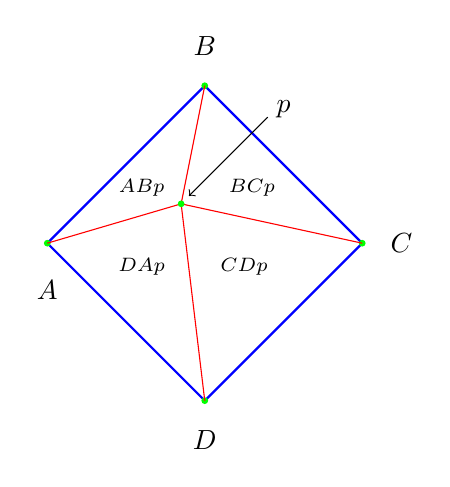
\begin{tikzpicture}
\draw[thick,blue] (0,0) -- (2,2) -- (4,0) -- (2,-2) -- cycle;

\filldraw[green] (0,0) circle(1pt);
\filldraw[green] (2,2) circle(1pt);
\filldraw[green] (4,0) circle(1pt);
\filldraw[green] (2,-2) circle(1pt);

\draw (0,-0.6) node {$A$};
\draw (2,2.5) node {$B$};
\draw (4.5,0) node {$C$};
\draw (2,-2.5) node {$D$};

\draw (3,1.7) node[fill=white] {$p$};
\draw[->] (2.8,1.6) -- (1.8,0.6);

\draw [red] (0,0) -- (1.7,0.5);
\draw [red] (2,2) -- (1.7,0.5);
\draw [red] (4,0) -- (1.7,0.5);
\draw [red] (2,-2) -- (1.7,0.5);

\filldraw[green] (1.7,0.5) circle(1pt);

\draw (1.2,0.7) node {$\scriptstyle ABp$};
\draw (2.6,0.7) node {$\scriptstyle BCp$};
\draw (2.5,-0.3) node {$\scriptstyle CDp$};
\draw (1.2,-0.3) node {$\scriptstyle DAp$};
\end{tikzpicture}
\end{minipage}
\begin{minipage}[h]{0.6\columnwidth}
La idea general es la siguiente: si un punto pertenece a una figura, y
construimos distintos triángulos con ese punto como uno de sus
vértices, la orientación de todos estos triángulos formados debe ser
la misma.

Por ejemplo en la figura de la izquierda, vemos como es importante el
orden en que se escogen los vértices de los triángulo. Deben escogerse
de modo que, si el punto efectivamente pertenece a la figura, todas
las orientaciones sean la misma, y en concreto, positiva. Para ello,
siempre hemos construido los triángulos en sentido horario y con el
punto $p$ como tercer vértice.
\end{minipage}

 Si por
ejemplo el segundo triángulo fuera $CBp$ en vez de $BCp$, el módulo de
su producto vectorial sería positivo, y por lo tanto su orientación
negativa, y nuestro método no funcionaría: el resto de triángulos
tendría una orientación positiva, sus orientaciones serían distintas,
y se nos indicaría que el punto no pertenece a la figura, lo cual es
falso.

Aquí se hace evidente por qué decidimos dar una orientación positiva
al caso $|\vec{u}\times\vec{v}| = 0$. En este caso, en nuestra
construcción de la figura, implicaría que el punto $p$ pertenece a una
arista (la correspondiente al triángulo construido actualmente) o
incluso a un vértice, y un punto que pertenece a una arista o un
vértice de la figura pertenece a la propia figura.

Es fácil ver como este método es aplicable directamente a cualquier
problema de pertenencia de un punto a un poliedro, su cálculo es muy
sencillo y computacionalmente es muy óptimo, pues su coste asintótico
es lineal respecto al número de vértices de la figura (dado que para
$n$ vértices, hay que construir $n$ triángulos y calcular el sentido
de cada uno de ellos).

Este problema me resulta importante por ser el primer problema
geométrico con el que me tuve que enfrentar en el juego, preparando
terreno para lo que vendría a continuación. Tras esto, se creó un
conjunto de estructuras y funciones que resolvían muchos otros
problemas geométricos necesarios, algunos sencillos de crear y otros
necesitando calma y tiempo para encontrar una solución correcta y
potente; cabe mencionar aquí el trato de rectas (caracterizadas como
hiperplanos) y el trato con circunferencias (sobre todo sobre la
intersección de circunferencias).

\subsection{Capacidades de movimiento actual}
El mundo de la intersección vino a tomar forma viva en este
problema. Tenemos tres casos del mismo: movimiento \emph{rect} máximo,
pivotaje derecho máximo, y pivotaje izquierdo máximo.

Tales problemas vienen delimitados por una máxima: no podrás acercarte
a menos de 10 unidades de terreno (véase reglamento) de otra unidad, sea amiga o
enemiga, y esto añade una dificultad interesante en el caso de los
pivotajes.

\subsubsection{Desplazamiento máximo}
En este problema se debe conseguir saber cual es la longitud máxima
que puede desplazarse una unidad en linea recta. Una unidad dispone de
un desplazamiento máximo de partida, y se ha de saber si existen
unidades en el camino que dificulten recorrer ese desplazamiento
máximo, teniendo en cuenta la distancia de respeto de 10 unidades de
terreno de juego entre unidades del mismo o distinto bando.

El problema se caracteriza de la siguiente forma: se construye un
rectángulo que tenga por ancho el frente de la unidad, y por alto, el
desplazamiento máximo de la unidad. Ahora se ha de ver qué unidades
enemigas tienen intersección con ese rectángulo (una unidad no es más
que otro rectángulo que caracteriza su ubicación), e ir calculando el
rectángulo libre de máxima altura a partir del rectángulo original.

Dos figuras pueden estar en posición una respecto a la otra de las
siguientes formas:
\begin{itemize}
\item Figuras disjuntas: cuando no tienen intersección.
\item Figuras contenidas: cuando su intersección es uno de los dos
  rectángulos.
\item Figuras cruzadas: cuando los vértices de su intersección no son
  vértices de ninguno de los dos rectángulos.
\item Figuras secantes: cuando su intersección contiene vértices
  de alguno de los dos rectángulos.
\end{itemize}

Esta taxonomía es importante por los siguientes motivos:
\begin{itemize}
\item Si buscamos vértices de otra figura, que pertenezcan a un
  dada, estoy encontrando figuras secantes y contenidas.
\item Si busco intersecciones de aristas, encuentro figuras secantes y cruzadas.
\item En caso contrario, las figuras son independientes.
\end{itemize}

Además, partimos del hecho de que la unidad de origen es una figura
\emph{bien colocada}. Con esto quiero decir que como partida la unidad
es disjunta a cualquier otra, y además, con 10 unidades de terreno de
separación, por lo tanto, el rectángulo de desplazamiento no estará
nunca contenida en ninguna otra figura, y nunca tendré que buscar que
sus vértices pertenezcan a las restantes.

\begin{minipage}[h]{0.4\columnwidth}
\centering
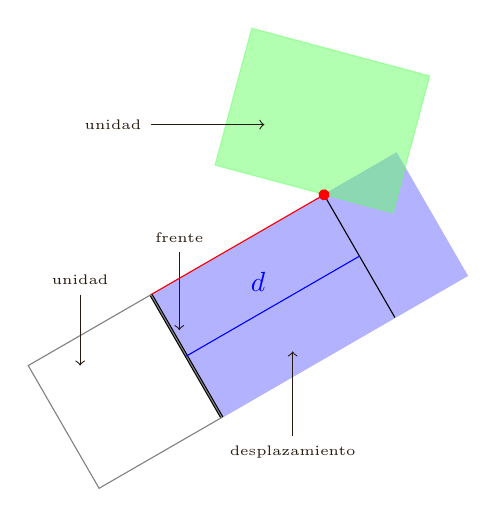
\begin{tikzpicture}[scale=1.8]
\filldraw[rotate=300,blue!30] (0,0) -- (1,0) -- (1,2) -- (0,2) --
cycle;
\filldraw[rotate=300,very thick] (0,0) -- (1,0);
\draw[brown!20!black,->] (.2,.3) node[above] {\tiny{frente}} -- (0.2,-.25);
\filldraw[rotate=345,opacity=.5, green!60] (0.2,1) -- (1.5,1) -- (1.5,2) -- (0.2,2) -- cycle;
\draw[rotate=300,gray,thin] (0,0) -- (1,0) -- (1,-1) -- (0,-1) --
cycle;
\draw[rotate=30,red] (0,0) -- (1.41,0);
\draw[rotate=30,black] (1.41,0)  -- (1.41,-1);
\draw[rotate=30,blue] (0,-0.5) -- (1.41,-0.5);
\draw[rotate=30,blue] (0.7,-0.3) node {$d$};
\filldraw[red,rotate=30] (1.41,0) circle(1pt);
\draw[brown!20!black,->] (-.5, 0) node[above] {\tiny{unidad}} -- (-.5, -.5);
\draw[brown!20!black,->] (1,-1) node[below] {\tiny{desplazamiento}}  --
(1,-.4);
\draw[brown!20!black,->] (0,1.2) node[left] {\tiny{unidad}} -- (.8,1.2);
\end{tikzpicture}
\end{minipage}
\begin{minipage}[h]{0.6\columnwidth}
Como podemos observar en la figura de la izquierda, para una unidad y
una arista concreta, hallamos la distancia de la
intersección entre la arista izquierda del área de desplazamiento y la
arista de la unidad \emph{enemiga}, hasta el frente de la unidad a
desplazar. Esa distancia será una cota máxima de desplazamiento
durante el resto del proceso de búsqueda.

Y este procedimiento se ejecuta para cada intersección entre cada
arista de cada unidad enemiga y las dos aristas verticales del área de
desplazamiento, y para cada vértice dentro del área de desplazamiento,
buscando el conflicto de menor distancia hasta el frente. También
ejecutamos estas operaciones con los bordes del escenario.
\end{minipage}

Hace falta advertir que al principio del proceso de búsqueda, se
ensancha virtualmente la unidad a desplazar un total de 10 unidades de
terreno, a lo ancho y a
lo alto, para respetar la distancia entre unidades de forma intrínseca
a la búsqueda.

\subsubsection{Pivotaje máximo}
De forma análoga al caso anterior, para calcular el pivotaje máximo
(por ejemplo, el pivotaje izquierdo -es decir, manteniendo como eje de
giro la esquina superior izquierda de la unidad-) ejecutamos de forma
similar al problema anterior, pero esta vez, en vez de trabajar con rectángulos, se trabaja
con una semicircunferencia que marca el pivotaje máximo inicial, y a
partir de ahí, reducimos el posible ángulo de giro a medida que se
encuentren intersecciones con otras unidades.

Pero como dijimos antes, aquí el hecho de engrosar a la unidad 10
unidades de terreno no nos da ninguna ventaja, y esta restricción hay
que cuidarla explícitamente en el proceso de búsqueda. El hecho de que
no nos de ninguna ventaja es debido a que, primeramente, el radio de
la semicircunferencia de partida no es el ancho de la unidad, sino su
diagonal.

Dado que al desplazar la unidad, hay que tener en cuenta el terreno
que este ocupa, también por ello hay que considerar la esquina opuesta al
eje de pivotaje, que siempre quedará fuera de dicha
semicircunferencia, como se aprecia en la figura inferior.

Por ello, como se ve en el gráfico, el área correcta de consideración es la
semicircunferencia de radio igual a la diagonal de la unidad. Y esta
diagonal no tiene ninguna relación ni proporción directa con las diez
unidades de terreno que se intentan respetar ensanchando a la unidad.

\begin{minipage}[h]{.5\columnwidth}
Por otro lado, ahora estamos calculando ángulos, no distancias. Un
incremento de 10 unidades de terreno en altura, son las 10 unidades de
terreno que hay que respetar si el movimiento es recto. Pero como
ahora tratamos con giros, un incremento de 10 unidades de terreno no
implican una distancia de 10 unidades de terreno con el punto de
intersección de dicha semicircunferencia con otra unidad. Así que,
ahora debemos de recurrir a otra solución para conseguir ese
\emph{respeto}.
\end{minipage}
\begin{minipage}[h]{.5\columnwidth}
\centering
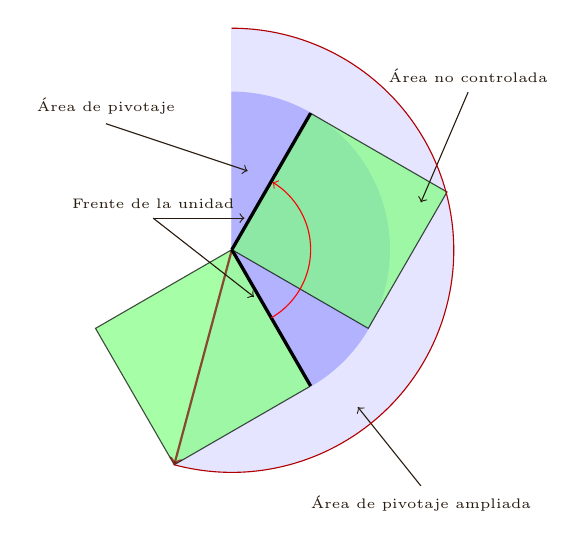
\begin{tikzpicture}[scale=2]
\filldraw[blue!10,rotate=300] (0,0) -- (1,-1) arc (-45:150:1.41cm) --
cycle;
\filldraw[opacity=.7,rotate=300,green!50,draw=black] (0,0) -- (1,0) --
(1,-1) -- (0,-1) -- cycle;
\draw[opacity=.7,red!50!black,rotate=300,thick,->] (0,0) -- (1,-1);
\filldraw[blue!30,rotate=300] (1,0) arc (0:150:1cm) -- (0,0) -- cycle;
\filldraw[very thick,rotate=300] (0,0) -- (1,0);

\filldraw[opacity=.7,rotate=60,green!50,draw=black] (0,0) -- (1,0) -- (1,-1) -- (0,-1) --
cycle;
\draw[red,->,rotate=300] (.5,0) arc (0:119:.5cm);
\filldraw[very thick, rotate=60] (0,0) -- (1,0);
\draw[brown!20!black,->] (-.8,.8) node[above] {\tiny{Área de pivotaje}}
-- (.1,.5);
\draw[brown!20!black,->] (1.2,-1.5) node[below] {\tiny{Área de pivotaje ampliada}}
-- (.8,-1);
\draw[brown!20!black,->] (1.5,1) node[above] {\tiny{Área no controlada}}
  -- (1.2,.3);
\draw[red!70!black,rotate=300] (1,-1) arc (-45:150:1.41cm);
\draw[brown!20!black,->] (-.5,.2) node[above] {\tiny{Frente de la unidad}}
  -- (.08,.2);
\draw[brown!20!black,->] (-.5,.2) -- (.14,-.3);
\end{tikzpicture}
\end{minipage}

\begin{minipage}[h]{0.5\columnwidth}
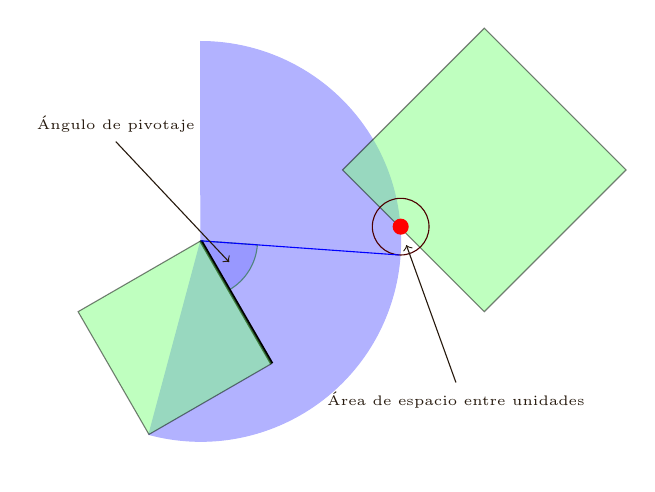
\begin{tikzpicture}[scale=1.8]
\filldraw[blue!30,rotate=300] (0,0) -- (1,-1) arc (-45:150:1.41cm) --
cycle;
\filldraw[opacity=.5,blue!50, draw=green!40!black,rotate=300] (.4,0) arc(0:56:.4cm) -- (0,0) -- cycle;
\draw[very thick, rotate=300] (0,0) -- (1,0);
\filldraw[opacity=.5,rotate=300,green!50,draw=black] (0,0) -- (1,0) --
(1,-1) -- (0,-1) -- cycle;
\filldraw[opacity=.5,green!50,draw=black] (1,.5) -- (2,1.5) --
(3,0.5) -- (2,-.5) -- cycle;
\filldraw[red] (1.41,.1) circle(1.5pt);
\draw[red!30!black] (1.41,.1) circle(.2cm);
\draw[blue] (0,0) -- (1.4,-.1);

\draw[brown!20!black,->] (1.8,-1) node[below] {\tiny{Área de espacio
    entre unidades}}-- (1.45,-.03);
\draw[brown!20!black,->] (-.6,.7) node[above] {\tiny{Ángulo de pivotaje}}-- (.2,-.15);
\end{tikzpicture}
\end{minipage}
\begin{minipage}[h]{0.5\columnwidth}
La solución adoptada es la siguiente: al igual que en el caso
anterior, para cada unidad, encontramos la intersección entre sus
aristas y la semicircunferencia de referencia de pivotaje, y también
los puntos que estén dentro de la figura. Y ahora, para cada punto,
trazamos una circunferencia de un radio de 10 unidades de
terreno. Luego tomamos los dos puntos de intersección entre dicha
circunferencia y la semicircunferencia de pivotaje: si se traza una
recta desde el origen de la semicircunferencia a dichos puntos, éstos
serán tangentes a la circunferencia \emph{de precaución}, y son éstos
puntos precisamente los que nos interesan.
\end{minipage}

De esta forma, buscamos el punto que nos de un ángulo de pivotaje
mínimo, y ese será el ángulo disponible de pivotaje actualmente.

Hay que advertir que, aunque nunca nos puede dar un ángulo
menor que 45º (puesto que la semicircunferencia de pivotaje tiene esta
cota mínima), si el valor está comprendido entre 0 y -45 (aunque
estrictamente hablando, esto no es un ángulo de pivotaje), significará
que la unidad no puede moverse porque si pivotara, entraría en
contacto con una unidad que está a su lado, pero no delante.

\subsection{Visión de una unidad}
Caracterizar la visión de una unidad, es decir, determinar qué unidad
ve a quién, es igual que caracterizar la
visión de una persona. Una persona ve un objeto cuando el espacio que
hay entre los dos está completamente libre. Si está parcialmente
ocupado también puede observarse dicho objeto, aunque la calidad de la
información que se recibe de dicho objeto es bastante menor. Si la parcialidad
de la obstaculización es muy alta, llegando a ocultar casi la
totalidad del objeto, se observará una figura de la que no
se reconocerá su forma, es decir, no se sabrá que objeto es.

Al principio, el problema de la caracterización de una unidad ignoraba
este último detalle tan importante y la vez tan simplificador. Se
intentó programar un algoritmo que admitiera una visualización directa
con tal de que el espacio no estuviera \emph{completamente}
ocupado. Es decir, que una sola recta infinitesimal de visión era
suficiente. La única forma de determinar tal tipo de visualización era
modificando el área de visión de partida.

Es decir, si partíamos de una semicircunferencia con centro en la
unidad y una amplitud de 120º de visión (siempre respecto al frente de
la unidad, porque es el frente el \emph{que ve}). Esta figura debe
entonces poderse modificar en otra figura de la complejidad que sea,
incluso dividirse en varias figuras disjuntas. Por ejemplo, un objeto
frente a la unidad de origen parte el área de visión en dos: la visión
correspondiente a los efectivos situados mas a la izquierda de la
unidad, y la visión correspondiente a los efectivos situados mas a la
derecha. Por tanto, determinar si la unidad objetivo es vista es
dividida en la determinación de la \emph{supervivencia} de dos
áreas. Si imaginamos todas las posibles situaciones nos damos cuenta
de que nos podemos encontrar ante cualquier tipo de partición y de
figura geométrica imaginable.

\begin{minipage}[h]{0.5\columnwidth}
Cuando se tuvo en cuenta el hecho de que, para observar un objeto, al
menos debe haber una franja continua de visionado, el problema se
simplificó de la siguiente forma: en vez de tener el problema de un
área modificable, y pretender que ese área nunca se haga nula (lo que
implicaría que no existe visibilidad), ahora lo resolvemos con un
descarte de áreas.

Cada área será lo que en la figura de nuestra derecha hemos llamado
\emph{haz de visión}. Un haz de visión es un rectángulo que comienza
en el frente de la unidad origen, y finaliza en una arista de la unidad de destino.
\end{minipage}
\begin{minipage}[h]{0.5\columnwidth}
\centering
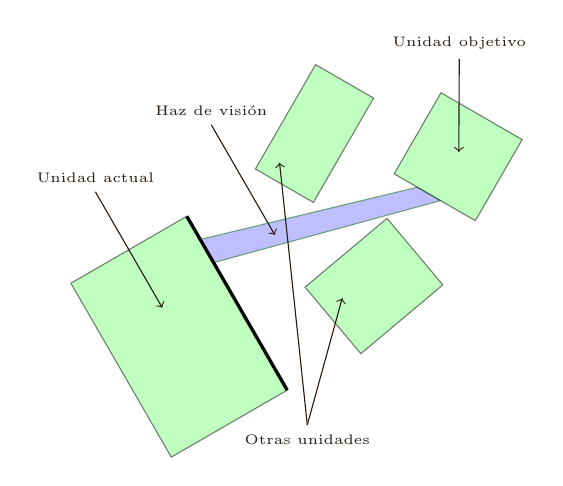
\begin{tikzpicture}[
  scale=1.7,
  rotate=300,
  unidad/.style={opacity=.5,green!50,draw=black},
  area/.style={opacity=.5,blue!50, draw=green!40!black},
  descripcion/.style={brown!20!black,->},
  ]
\coordinate (A) at (0,1);
\coordinate (B) at (1.5,1);
\coordinate (C) at (1.5,0);
\coordinate (D) at (0,0);

\coordinate (a) at (.5,2.5);
\coordinate (b) at (1.2,2.5);
\coordinate (c) at (1.2,3.2);
\coordinate (d) at (.5,3.2);

\coordinate (REF) at (a);
\coordinate (CENTRO) at (.75,1);

\filldraw[area] (0.4,1) -- (0.2,1) -- ({.5 + .2*cos(30)}, {2.5 + .2*sin(30)})--
+({.2*cos(30)}, {.2*sin(30)}) -- cycle;

\filldraw[unidad] (A) rectangle (C);

%No se por que no funciona girar coordenadas (c).
\filldraw[unidad,rotate around={30:(REF)}] (a) rectangle (1.2,3.2);

\coordinate (alfa) at (.9,1.5);
\coordinate (beta) at (1.4,2.4);

\filldraw[unidad,rotate around={10:(alfa)}] (alfa) rectangle (beta);

\filldraw[unidad,rotate around={30:(-.5,2.4)}] (0,1.5) rectangle
(-.5,2.4);

\draw[descripcion] (-.5,.5) node[above]{\tiny{Unidad actual}} --
(.5,.5);
\draw[descripcion] (-.5,1.5) node[above]{\tiny{Haz de visión}} --
(.45,1.5);

\coordinate (refunidades) at (1.8,1);

\draw[descripcion] (refunidades) node[below]{\tiny{Otras unidades}} --
(1.11,1.7);

\draw[descripcion] (refunidades) -- (0,1.8);

\draw[very thick] (A) -- (B);

\coordinate (refunidadobjetivo) at (0,3.35);

\draw[descripcion] (refunidadobjetivo) node[above]{\tiny{Unidad
    objetivo}} -- (.6,3);
\end{tikzpicture}
\end{minipage}

Tanto la base, en la unidad de origen, como su arista opuesta en la
unidad de destino, tienen un tamaño de 5 unidades de terreno, pues
esta ha sido la cota elegida para caracterizar la visión de una
unidad.

Lo que hacemos, en general, es crear todos los
posibles haces de visión entre la unidad origen y la unidad
objetivo. Esto entraña un problema. Por ejemplo, si nos fijamos en la
figura de referencia, la unidad de origen podrá ver, como mucho, dos
aristas de la unidad de destino. El nuevo problema que surge con este
planteamiento es el de caracterizar la arista o aristas
características de visión. Este problema se resuelve tal y como
muestra la siguiente figura.

\begin{minipage}[h]{0.4\columnwidth}
\centering
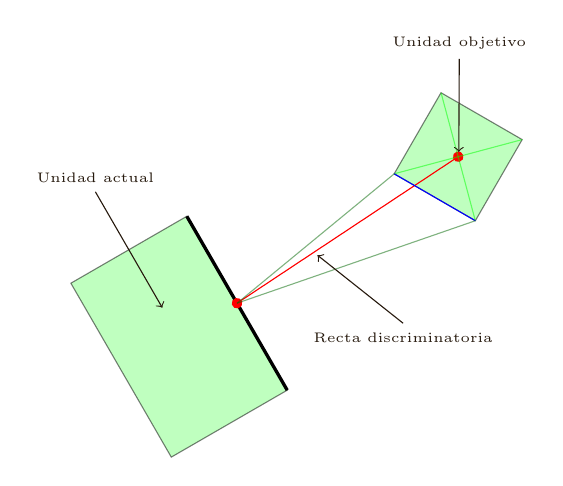
\begin{tikzpicture}[
  scale=1.7,
  rotate=300,
  unidad/.style={opacity=.5,green!50,draw=black},
  area/.style={opacity=.5,blue!50, draw=green!40!black},
  descripcion/.style={brown!20!black,->}
  ]
\coordinate (A) at (0,1);
\coordinate (B) at (1.5,1);
\coordinate (C) at (1.5,0);
\coordinate (D) at (0,0);

\coordinate (a) at (.5,2.5);
\coordinate (b) at (1.2,2.5);
\coordinate (c) at (1.2,3.2);
\coordinate (d) at (.5,3.2);

\coordinate (REF) at (a);
\coordinate (CENTRO) at (.75,1);

\filldraw[unidad] (A) rectangle (C);

%No se por que no funcioan girar coordenadas (c) no funciona.
\filldraw[unidad,rotate around={30:(REF)}] (a) rectangle (1.2,3.2);
\draw[very thick] (A)--(B);

\filldraw[red,rotate around={30:(REF)}] (CENTRO) circle(1pt) -- (intersection of a--1.2,3.2
and 1.2,2.5--.5,3.2) circle(1pt);
\draw[opacity=.5,green, rotate around={30:(REF)}] (a)--(1.2,3.2);
\draw[opacity=.5,green, rotate around={30:(REF)}] (1.2,2.5)--(.5,3.2);

\draw[blue, rotate around={30:(REF)}] (a)--(1.2,2.5);
\draw[area] (CENTRO)--(a);
\draw[area, rotate around={30:(REF)}] (CENTRO) -- (1.2,2.5);

\draw[descripcion] (-.5,.5) node[above]{\tiny{Unidad actual}} --
(.5,.5);

\coordinate (refunidadobjetivo) at (0,3.35);

\draw[descripcion] (refunidadobjetivo) node[above]{\tiny{Unidad
    objetivo}} -- (.6,3);

\draw[descripcion] (1.5,2) node[below]{\tiny{Recta discriminatoria}}
-- (.74, 1.7);
\end{tikzpicture}

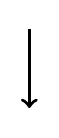
\begin{tikzpicture}
\draw[very thick, black, ->] (5,1) -- (5,0);
\end{tikzpicture}

\begin{tikzpicture}[
  scale=1.7,
  rotate=300,
  unidad/.style={opacity=.5,green!50,draw=black},
  area/.style={opacity=.5,blue!50, draw=green!40!black},
  descripcion/.style={brown!20!black,->},
  decoration = {
    markings,
    mark=at position .50 with {\arrow[red, line width = 1.5pt]{>};} }
  ]
\coordinate (A) at (0,1);
\coordinate (B) at (1.5,1);
\coordinate (C) at (1.5,0);
\coordinate (D) at (0,0);

\coordinate (a) at (.5,2.5);
\coordinate (b) at (1.2,2.5);
\coordinate (c) at (1.2,3.2);
\coordinate (d) at (.5,3.2);

\coordinate (REF) at (a);
\coordinate (CENTRO) at (.75,1);

\filldraw[area,opacity=.3,rotate around={30:(REF)}] (CENTRO) -- (.5,3.2) --
(1.2,2.5) -- cycle;
\filldraw[area,black!80,rotate around={30:(REF)}] (.5,3.2) --
(1.2,2.5) -- (1.2,3.2) -- cycle;

\filldraw[unidad] (A) rectangle (C);

%No se por que no funcioan girar coordenadas (c) no funciona.
\filldraw[unidad,rotate around={30:(REF)}] (a) rectangle (1.2,3.2);
\draw[very thick] (A)--(B);

\draw[red, rotate around={30:(REF)}] (1.2,2.5)--(.5,3.2);

\draw[blue, rotate around={30:(REF)}] (a)--(1.2,2.5);
\draw[blue, rotate around={30:(REF)}] (a)--(.5,3.2);
\draw[red, rotate around={30:(REF)},postaction={decorate}] (CENTRO) --
(1.2,2.5);

\draw[descripcion] (1.5,2) node[below]{\tiny{Área de referencia}}
-- (.74, 2);
\draw[descripcion] (0,3.5) node[above]{\tiny{Área oculta}} --
(.6,3.15);
\draw[descripcion] (-.27,1.4) node[above]{\tiny{Diagonal
    discriminatoria}} -- (.63,2.96);
\end{tikzpicture}
\end{minipage}
\begin{minipage}[h]{0.6\columnwidth}
Proyectamos, desde el centro del frente de la unidad de origen, un
segmento que acabe en el centro del rectángulo de la unidad de
destino. A esa recta la llamaremos recta discriminatoria. Esa recta
deberá intersecar con alguna arista de la unidad de
destino. A esa arista la llamaremos arista discriminatoria.

Luego, desde el centro del frente, proyectamos dos nuevos segmentos,
que acaben respectivamente en los extremos de la arista
discriminatoria. Nos quedamos, en este caso, con el segmento de mayor
longitud, situación que nos lleva a la segunda figura.

Una vez determinado el segmento mayor, elegimos la diagonal de la
unidad enemiga que coincida con su extremo con dicho segmento. A esta
diagonal la llamaremos, finalmente, diagonal discriminatoria.

Esta diagonal es importante porque divide a la unidad objetivo en dos
mitades, una que está frente a la unidad origen, y otra que
está \emph{oculta}. Las aristas que estén delante de la diagonal
discriminatoria serán las que queden descubiertas a la unidad
origen. Se puede observar como estas aristas están dentro del
\emph{área de referencia} que hemos construido proyectando el centro
del frente ha la diagonal discriminatoria.
\end{minipage}

Y ahora hacemos la última observación importante. Si intentamos
construir todos los haces de visión posibles con respecto a las
aristas descubiertas, y también, y ésta es la novedad, con respecto a la diagonal de
referencia, nos damos cuenta de que, con solo hacer que la unidad vea
a la diagonal de referencia, nos basta para admitir que ve a la unidad
original.

El método, pues, será explorar una a una todas las unidades de la
partida (de media, unas 10 o 15 unidades)
para cada rectángulo de referencia (que de media, serán entorno a unas
60), buscando intersecciones que descarten a dichos rectángulos, y, en
cuanto encontremos un haz de visión libre, abortamos la búsqueda y
admitimos que la unidad de origen vé a la unidad de destino.

\subsection{Movimiento de carga}
El movimiento de carga se resuelve de forma muy parecida al problema
de la visión, al menos en su planteamiento inicial. Evidentemente,
para cargar, la unidad tiene que ver a su objetivo. Y además, solo
podrá cargar a uno de los flancos que estén dentro de su 
visión. Y en este sentido, es donde se reenlaza este problema con el
anterior:

\begin{itemize}
\item Se obtienen las aristas \emph{descubiertas} vistas en la sección
  anterior.
\item Se buscan todas las posibles posiciones de carga en dichas
  aristas.
\item Se asegura que una posición sea accesible mediante una carga.
\item Se sigue buscando hasta encontrar una posición que también sea
  accesible, y que sea mejor, usando los criterios impuestos por el
  reglamento de \gom sobre los movimientos de carga.
\item Se desplaza la unidad a dicha posición.
\end{itemize}

Las distintas posiciones en las que es posible efectuar una carga
también es similar al caso anterior. En cada arista descubierta, voy
\emph{deslizando} un segmento del mismo tamaño que el frente de la
unidad, a intervalos de 5 en 5 unidades de terreno. Cada posición,
representa una posible posición de carga. Además, como los rangos de
ocupacion de las unidades son siempre múltiplos de 5, de esta forma se
exploran todas las posibles situaciones útiles.

Para calcular si el espacio de carga está disponible, sencillamente,
formamos un rectángulo como resultado de unir los extremos de ambos
segmentos: el frente de la unidad, y el nuevo frente virtual de la
nueva y posible posición de carga. Si dicho rectángulo está libre y si
además, la posición final también lo está, diremos que la carga es
posible. Luego tendremos que vigilar si existen mas posiciones de
carga que permitan enfrentar un número mayor de efectivos, o que se
recorra una distancia menor.

Si bien es cierto que el movimiento de carga real de la unidad no tiene
por qué coincidir con el área marcada por el rectángulo que formamos para su
representación, no nos hace falta tener en cuenta la posible área de
la unidad que pueda salirse de dicho rectángulo, por las siguientes razones:

\begin{itemize}
\item Los movimientos de carga son movimientos en partes libres y
  caóticos, y no se puede caracterizar en qué posición exacta estaría
  cada unidad en cada paso de la carga.
\item Las unidades, en la antigüedad, podían reorganizarse y
  pivotar suavemente al inicio de la carga, se podia perder levemente
  la rigidez de la formación 
  formación para hacer mas flexible su recorrido, etc. Con esto, la
  unidad tiene cierta flexibilidad a la hora de desplazar su carga,
  siendo dicho \emph{área de carga} rectángulas la mejor aproximación
  a su recorrido.
\item Y la última razón, y a su vez la mas importante, ninguna
  posición intermedia en este \emph{área de carga} será
  una posición final de la unidad, salvo la última, y la última sí que
  se comprueba.
\end{itemize}

\subsection{Movimiento de huida}
El movimiento de huida se puede ver como una variante del problema del
desplazamiento con la diferencia o particularidad de que el
desplazamiento, en vez de tener una cota máxima de movimiento, su cota
es mínima.

Es decir, en el caso del desplazamiento, se debía calcular cual era el
desplazamiento máximo que se podía realizar sin entrar en contacto con
ninguna otra unidad. En el caso del movimiento de la huida, el valor
de partida es el valor mínimo que hay que realizar, y si no hay
espacio, este valor se supera en busca de la primera posición de la
unidad que tenga el suficiente espacio libre como para que la unidad
que huye pueda \emph{estacionar}.

En general, el verdadero problema es caracterizar la posición final de
la unidad cuando existen unidades que entorpecen la huida.

Para ello, supongamos que existen unidades en el camino de huida que no
nos permiten detener a la unidad en el lugar que le corresponde según
la cantidad de movimiento de huida asignado.

Como se observa en la figura inferior, si intentasemos colocar a la
unidad en su posición adjudicada, que en la figura hemos llamado
límite de huida, la unidad se colocaría justo encima de la primera
unidad foránea existente en el camino. Tal y como indica el
reglamento, la unidad debe continuar su movimiento hasta encontrar la
primera posición libre.

\begin{minipage}[h]{.5\columnwidth}
Para ello, en cada unidad presente en el camino, trazamos un par de
rectas discriminantes para cada unidad, una justo delante suya, que
llamaremos proximal, y otra justo detrás suya, que llamaremos recta
distal. Son las que hemos puesto de color rojo en la
figura.

Para cada unidad, obtenemos el espacio que existe entre la recta
distal de la primera unidad y la recta proximal de la siguiente,
restandole 20 unidades de terreno a dicha distancia (10u por la
primera unidad, y 10u por la segunda, para respetar la distancia entre
unidades tal y como exige el reglamento de \gomf).
Si esta distancia
es mayor a la profundidad de la unidad, significará que la 
unidad cabe en dicho espacio, y la primera posición encontrada que
cumpla con estas propiedades será la posición elegida final para
colocar a la unidad que está huyendo.
\end{minipage}
\begin{minipage}[h]{.5\columnwidth}
\centering
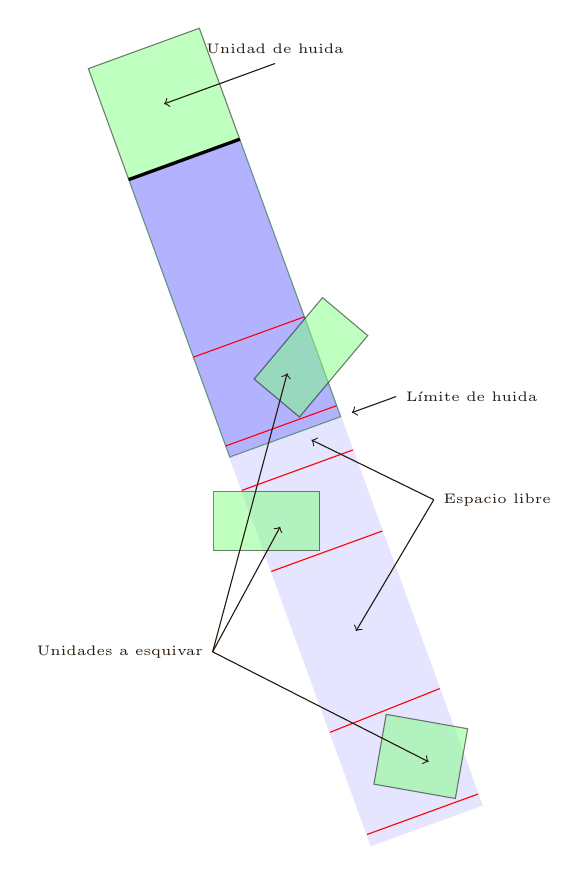
\begin{tikzpicture}[
  scale=1.5,
  rotate=200,
  unidad/.style={opacity=.5,green!50,draw=black},
  area/.style={opacity=.5,blue!50, draw=green!40!black},
  fondo/.style={blue!10},
  descripcion/.style={brown!20!black,->}
  ]

\filldraw[fondo] (0,1) rectangle (1,7);
\filldraw[area] (0,1) rectangle (1,3.5);
\filldraw[unidad] (0,0) rectangle (1,1);
\draw[very thick] (0,1) -- (1,1);
\filldraw[unidad, rotate around={30:(-.2,2.5)}] (-.2,2.5) rectangle
(.7,3);
\filldraw[unidad, rotate around={160:(1.4,4.2)}] (1.4,4.2) rectangle
(2.3,4.7);
\filldraw[unidad, rotate around={150:(.5,6)}] (.5,6) rectangle
(1.2,5.4);

\draw[red] (0,2.6) -- (1,2.6);
\draw[red] (0,3.4) -- (1,3.4);
\draw[red] (0,3.8) -- (1,3.8);
\draw[red] (0,4.53) -- (1,4.53);
\draw[red] (0,5.95) -- (1,5.98);
\draw[red] (0,6.9) -- (1,6.9);

\draw[descripcion] (-.5,.5) node[above]{\tiny{Unidad de huida}} --
(.5,.5);
\draw[descripcion] (-.5,4.43) node[right]{\tiny{Espacio libre}}
-- (.3,3.6);
\draw[descripcion] (-.5,4.43) -- (.5,5.25);
\draw[descripcion] (1.7,5) node[left]{\tiny{Unidades a esquivar}} --
(.3, 6.5);
\draw[descripcion] (1.7,5) -- (.8,4.2);
\draw[descripcion] (1.7,5) -- (.3,3);
\draw[descripcion] (-.5,3.5) node[right]{\tiny{Límite de huida}}--
(-.1,3.5);
\end{tikzpicture}
\end{minipage}
\cleardoublepage

% Este archivo es parte de la memoria del proyecto fin de carrera
% de Aarón Bueno Villares. Protegida bajo la licencia GFDL.
%
% Para más información, la licencia completa viene incluida en el
% fichero fdl-1.3.tex

% Copyright (C) 2010 Aarón Bueno Villares

\section{Pruebas}
\label{sec:pruebas}

Para diseñar los casos de prueba, distinguimos entre aquellas clases y
estructuras que, por su naturaleza, pueden ser testeadas
individualmente, de aquellas que se testean de forma integrada. La
mayoría de las funciones ofrecidas por el gestor de escenario fueron
testeadas de forma individual, al igual que todas las
estructuras matemáticas. En cambio, el resto de clases y funciones,
por su simplicidad y por su dependencia gráfica, no merecía la pena
realizar casos de prueba individuales, quizás mas complejos que
estudiar, simplemente, su comportamiento integrado. Así que, en
definitiva, la organización de los casos de prueba fue la siguiente:

\begin{enumerate}
\item A medida que se fueron implementando, se probaron
  individualmente todas las estructuras y funciones matemáticas
  diseñadas y las funciones de corte mas matemático.
\item Una vez superados los test anteriores, y a medida que se
  agregaba nueva funcionalidad, se probaba cada vez el sistema
  completo de forma integrada.
\item Al finalizar todo el proceso completo de diseño e implementación
  comenzaron las pruebas beta. Algunos usuarios probaron el producto y
  no se detectó ningún defecto adicional.
\end{enumerate}

\subsection{Pruebas alfa}
Las pruebas alfa son las pruebas que se realizan durante el proceso de
desarrollo. En el caso que nos ocupa, las pruebas se realizaban al
final de cada iteración de implementación.

\subsubsection{Pruebas unitarias}
Las funciones sustentas a este tipo de pruebas, como hemos dicho
antes, eran las mas relacionadas con el ámbito mas matemático del
juego. Debido a su complejidad, las pruebas se realizaron bajo un
enfoque estructural, es decir, de caja blanca, y además, bajo un
criterio de cobertura de sentencias, es decir, se estableció que la
mejor forma de estudiar el comportamiento correcto de una función era
lograr que al menos cada posible rama de la función fuese explorada,
con la finalidad de que al menos cada sentencia fuera ejecutada una
vez. A su vez, se diseñaron las pruebas de modo que las sentencias mas
problemáticas de cada función (aquellas que poseen divisiones,
peligros de desbordamiento, bucles o ecuaciones complejas) se probaran
varias veces explorando tanto los casos mas comunes como los mas
extremos (análisis de valores límite), de modo que se examine de forma
exhaustiva su comportamiento.

Como era de esperar, el mayor núcleo de errores de esta clase se
encontraban en la implementación de las estructuras matemáticas del
juego, que tenían alta implicación en el comportamiento del gestor de
escenarios.

\subsubsection{Pruebas de integración}
Las pruebas de integración del sistema complejo al completo (en cada
iteracción de diseño), debida a la relativa sencillez estructural de
las clases que la conformaban (una funcionalidad compleja pero formada
por un rico dinamismo de funciones individuales muy sencillas), se
realizaron bajo un enfoque funcional o de caja negra. Se probaba,
sencillamente, que la ejecución de la nueva funcionalidad
implementada, en consonancia con funcionalidades completadas previas,
realizara con éxito lo que se supone que debía realizar.

El principal núcleo de defectos encontrados bajo estas pruebas de
integración recayeron sobre el gestor de iconos, sobre el gestor de
ejércitos, y en los procesos de destrucción (cuando finaliza una
partida). 

\subsection{Pruebas beta}
Al finalizar el proceso de diseño, implementación y pruebas alfa se
ofreció el juego a distintos usuarios (generalmente compañeros de
universidad) para que probaran el juego y me remitieran los errores
producidos y el contexto del mismo. Luego repetía las situaciones
reportadas, hasta obtener el error nuevamente y explorar su origen,
corregir y reenviar la nueva versión a mis
\emph{ayudantes}. Generalmente, los fallos y defectos encontrados en
esta fase de pruebas fueron relacionadas con el proceso de huida de
las unidades desmoralizadas en combate.

\cleardoublepage

% Este archivo es parte de la memoria del proyecto fin de carrera
% de Aarón Bueno Villares. Protegida bajo la licencia GFDL.
%
% Para más información, la licencia completa viene incluida en el
% fichero fdl-1.3.tex

% Copyright (C) 2010 Aarón Bueno Villares

\section{Herramientas}
\label{sec:herramientas}

Para la realización de este proyecto se ha hecho uso de una serie de
herramientas y aplicaciones adicionales que facilitaron su desarrollo.

\subsection{GCC}
El proyecto ha sido desarrollado en el lenguaje de programación C++. Y
todo lenguaje necesita de un compilador que permita traducir el código
a código máquina, único lenguaje que la máquina comprende. Nuestro
particular traductor (mas concretamente, compilador) ha sido
GCC\footnote{\emph{GNU Compiler Collection.}}.

\emph{GCC} es un compilador de \emph{GNU}, por lo tanto libre y
abierto, que da soporte a varios lenguajes de programación, entre
ellos \emph{C++}. Pertenece al llamado \emph{GNU toolchain}, el
conjunto de herramientas de \emph{GNU} por y para la programación.
 
\subsection{libSDL}
Todo juego tiene una gran cantidad de elementos de interacción con el
usuario. Para ello, se debe tener acceso al hardware, de modo que
obtengamos información de todos los eventos de usuario producidos.

La librería SDL\footnote{\emph{Simple DirectMedia Layer.}} ha sido la
piedra angular del aspecto multimedia de nuestro juego. Lo hemos usado
principalmente para nuestra interacción con el sistema de video, y los eventos de teclado y
ratón. A su vez, hemos usado las siguientes librerias auxiliares de
\emph{SDL}:
\begin{description}
\item[SDL\_image:] Usado para la carga de imágenes (permite trabajar con
  imágenes de cualquier formato, mientras que \emph{SDL} solo permite
  cargar imagenes \emph{bmp}).
\item[SDL\_mixer:] Usado para nuestro trato con audio.
\item[SDL\_gfx:] Usado para rotar y redimensionar nuestras imágenes.
\item[SDL\_ttf:] Usado para imprimir texto en pantalla.
\end{description}

\subsection{GIMP}
\emph{GIMP}\footnote{\emph{GNU Image Manipulation Program.}} es otra
herramienta del proyecto \emph{GNU}. Como su nombre indica, es un
editor y manipulador de imágenes. Con él hemos creado (y/o modificado
a partir de otras imágenes libres) todos los iconos, los menus, las
peanas de las unidades, y en general, toda imagen y todo elemento
gráfico del juego a pasado por manos de \emph{GIMP}, bien para su
retoque, bien para su creación.

\subsection{GNU Emacs}
Richard Stallman junto a Guy Steele creó, en 1975,
el editor de textos Emacs\footnote{Editor MACroS}. Mas tarde, entre
1984 y 1985, se lanzó \emph{GNU Emacs}, una nueva versión derivada de
la anterior diseñada por Richard Stallman para el proyecto
\emph{GNU}. Hoy en día es considerada por muchos programadores como el
mejor editor de textos, y existen una gran diversidad de modos de
emacs que proveen diversos entornos de desarrollo para prácticamente
casi todos los lenguajes de programación.

Nuestro proyecto ha sido prácticamente desarrollado al completo en él.

\subsection{SVN}
Este proyecto dispone de un repositorio donde siempre hemos mantenido
actualizado el desarrollo del proyecto. \emph{SVN}\footnote{\emph{SubVersioN}.} ha sido la
herramienta auxiliar utilizada para interactuar con el repositorio,
actualizar las versiones, y mantener nuestra copia de seguridad del proyecto.

Las herramientas como \emph{SVN} proveen un mecanismo de control de
versiones cuando existen varios desarrolladores involucrados, evitando
que se destruyan cambios y ordenando las distintas modificaciones que
se van realizando en el proyecto, permitiendo tener acceso a
anteriores versiones de cada fichero involucrado en el proyecto, así
como del proyecto en su conjunto. Como este proyecto ha
sido desarrollado únicamente por mí, no se ha aprovechado
completamente la potencia de esta herramienta, pero aun así me ha
permitido tener acceso directo a mi proyecto desde cualquier máquina,
y tener acceso, además, a todas la versiones enviadas, que en varias
ocasiones me ha permitido recuperar versiones antiguas de ciertos
ficheros que he necesitado recuperar.

\subsection{Make}
\emph{Make} es una herramienta que hemos usado para la automatización
de la compilación del proyecto. \emph{Make} permite crear scripts,
comúnmente en un fichero llamado \emph{makefile}, para declarar las
dependencias de los distintos módulos, a fin de acelerar la
compilación (dependencias sin modificaciones no se recompilan) y
aumentar la robustez de la misma.

En nuestro proyecto, además de compilar el proyecto, a través de
\emph{make} podemos generar la documentación y la memoria del proyecto
(véase abajo), así como limpiar de forma directa todos los ficheros
intermedios e innecesarios creados en el proceso de compilación tanto
del proyecto como de la memoria.

\subsection{LaTeX}
\emph{TeX} fue concebido inicialmente por Donald Knuth a principios de la década de los
80 para construir un lenguaje de programación de edición
profesional de textos científicos, y ya en 1984 Leslie Lamport
desarrolló \emph{LaTeX} como un conjunto de macros que orientaban \emph{TeX}
a la edición de cartas, libros, y en general, a la edición de textos
desde un mayor nivel de abstracción.

Este proyecto ha hecho uso de este lenguaje para la construcción completa
de la memoria.

\subsection{Doxygen}
\emph{Doxygen} es una herramienta ideada para documentar código de
varios lenguajes de programación. Provee una serie de comandos, dentro
de los llamados \emph{comentarios de Doxygen}, que Doxygen sabe
interpretar y que luego usa para generar un documento html, pdf o rtf
(según los deseos del usuario) con la documentación del código,
haciendo uso además de \emph{Graphviz} y \emph{TeX} para generar gráficos de
dependencias entre clases y módulos, y proveer la inclusión de
fórmulas matemáticas en la documentación resultante.

Nuestro proyecto ha hecho uso de ésta herramienta para documentar el
código.

\subsection{Umbrello}
\emph{Umbrello} es una herramienta de apoyo para el desarrollo
software, sobre todo bajo un paradigma orientado a objetos, que
permite hacer un análisis y un diseño bajo el estándar UML, obtener
los diagramas UML mediante ingeniería inversa a partir de código
nativo, o automatizar parte de la implementación del software
creando el código a partir de los diagramas UML diseñados.

Se ha usado esta herramienta para realizar los diagramas UML de la
memoria.